% !TEX program = xelatex
\documentclass[hyperref,a4paper,UTF8]{ctexart}

\usepackage[left=2.50cm, right=2.50cm, top=2.50cm, bottom=2.50cm]{geometry}

\usepackage[unicode=true,colorlinks,urlcolor=blue,linkcolor=blue,bookmarksnumbered=true]{hyperref}
\usepackage{xcolor}
\usepackage{latexsym,amssymb,amsmath,amsbsy,amsopn,amstext,amsthm,amsxtra,color,bm,calc,ifpdf}
\usepackage{graphicx}
\usepackage{enumerate}
\usepackage{fancyhdr}
\usepackage{listings}
\usepackage{multirow}
\usepackage{makeidx}
\usepackage{fontspec}
\usepackage{subfigure}
\usepackage{hyperref}
\usepackage{pythonhighlight}
\usepackage{cite}
\usepackage[justification=centering]{caption}
\usepackage{pifont}
\usepackage{enumitem}
\usepackage{longtable}
\usepackage{makecell}
\usepackage{dirtree}
\usepackage{float}

\usepackage{tikz}
\usepackage{pgf-umlcd}
\usepackage{forest}
\usepackage{hyperref}

\lstset{
    language=Go, % 设置代码语言
    basicstyle=\small\ttfamily, % 设置基本字体样式
    commentstyle=\color{green!40!black}, % 设置注释样式
    keywordstyle=\color{blue}, % 设置关键字样式
    numberstyle=\tiny\color{gray}, % 设置行号样式
    numbers=left, % 行号位置
    frame=single, % 给代码添加边框
    breaklines=true, % 允许代码自动换行
    postbreak=\mbox{\textcolor{red}{$\hookrightarrow$}\space}, % 设置代码折行符号
    showstringspaces=false, % 不显示字符串中的空格
    captionpos=b, % 设置标题位置
    tabsize=4, % 设置制表符宽度
    morekeywords={as},
}


\pagestyle{fancy}
\fancyhead[L]{}
\fancyhead[C]{\fangsong  \quad FJE-GO:基于GO实现的JSON文件可视化工具}
\fancyhead[R]{}


\title{\vspace{3cm}\Huge\textbf{{ FJE-GO:基于GO实现的JSON文件可视化工具} \\ \LARGE{ }}\vspace{6cm}}


%这种书写格式感觉没有对齐
\author{
\kaishu\Large{姓名\ \ \ \ \underline{\  \ \ 李\ \ \ \ \ \ 博  \ \ \       }} \\\\
\kaishu\Large{学号\ \ \ \underline{2\ 1\ 3\ 0\ 7\ 2\ 7\ 8}} \\\\
\kaishu\Large{学院\ \ \ \underline{计\ 算\ 机\ 学\ 院}}\\\\
\kaishu\Large{专业\ \underline{计算机科学与技术}}
}






\date{} % 留空,不显示日期

\begin{document}

\begin{figure}
    \centering
    
\includegraphics[width=0.65\textwidth]{figures/sysu.png}
\end{figure}

\maketitle

\newpage


\tableofcontents 

\thispagestyle{empty} 


\section{项目代码}


\href{https://github.com/02lb/24SE-FJE}{【GitHub仓库链接】}

本项目使用的编程语言是GO语言,项目的源代码以及相关的测试文件、配置文件都已经在GitHub中给出,下面是整个项目的大致目录树以及文件的相关说明: \\


\dirtree{%
    .1 Design Pattern 习题(实验要求).
    .2 tex-report (实验报告).
    .2 src(源代码).
    .3 version-1 :第一版本代码.
    .3 verison-2 :基于设计模式以及实验要求优化后的第二版本代码.
    .4 component.go : 定义 Component 接口、Leaf 和 Container 类.
    .4 factory.go : 定义 Factory 接口及其具体实现.
    .4 builder.go : 定义 Builder 类.
    .4 explorer.go : 定义 FunnyJSONExplorer 类.
    .4 main.go : 主程序入口.
    .4 loadConfig.go : 定义处理Icon配置文件的相关类.
    .4 treeDraw.go : 实现对于 tree 风格的 Draw 方法.
    .4 rectangleDraw.go : 实现对于 rectangle 风格的 Draw 方法.
    .3 json : 用于测试的JSON文件.
    .3 config : 配置文件,可以用于 IconFamily 的配置.
}



\section{设计文档}

\subsection{类图与说明}

\begin{figure}[H]
    \centering
    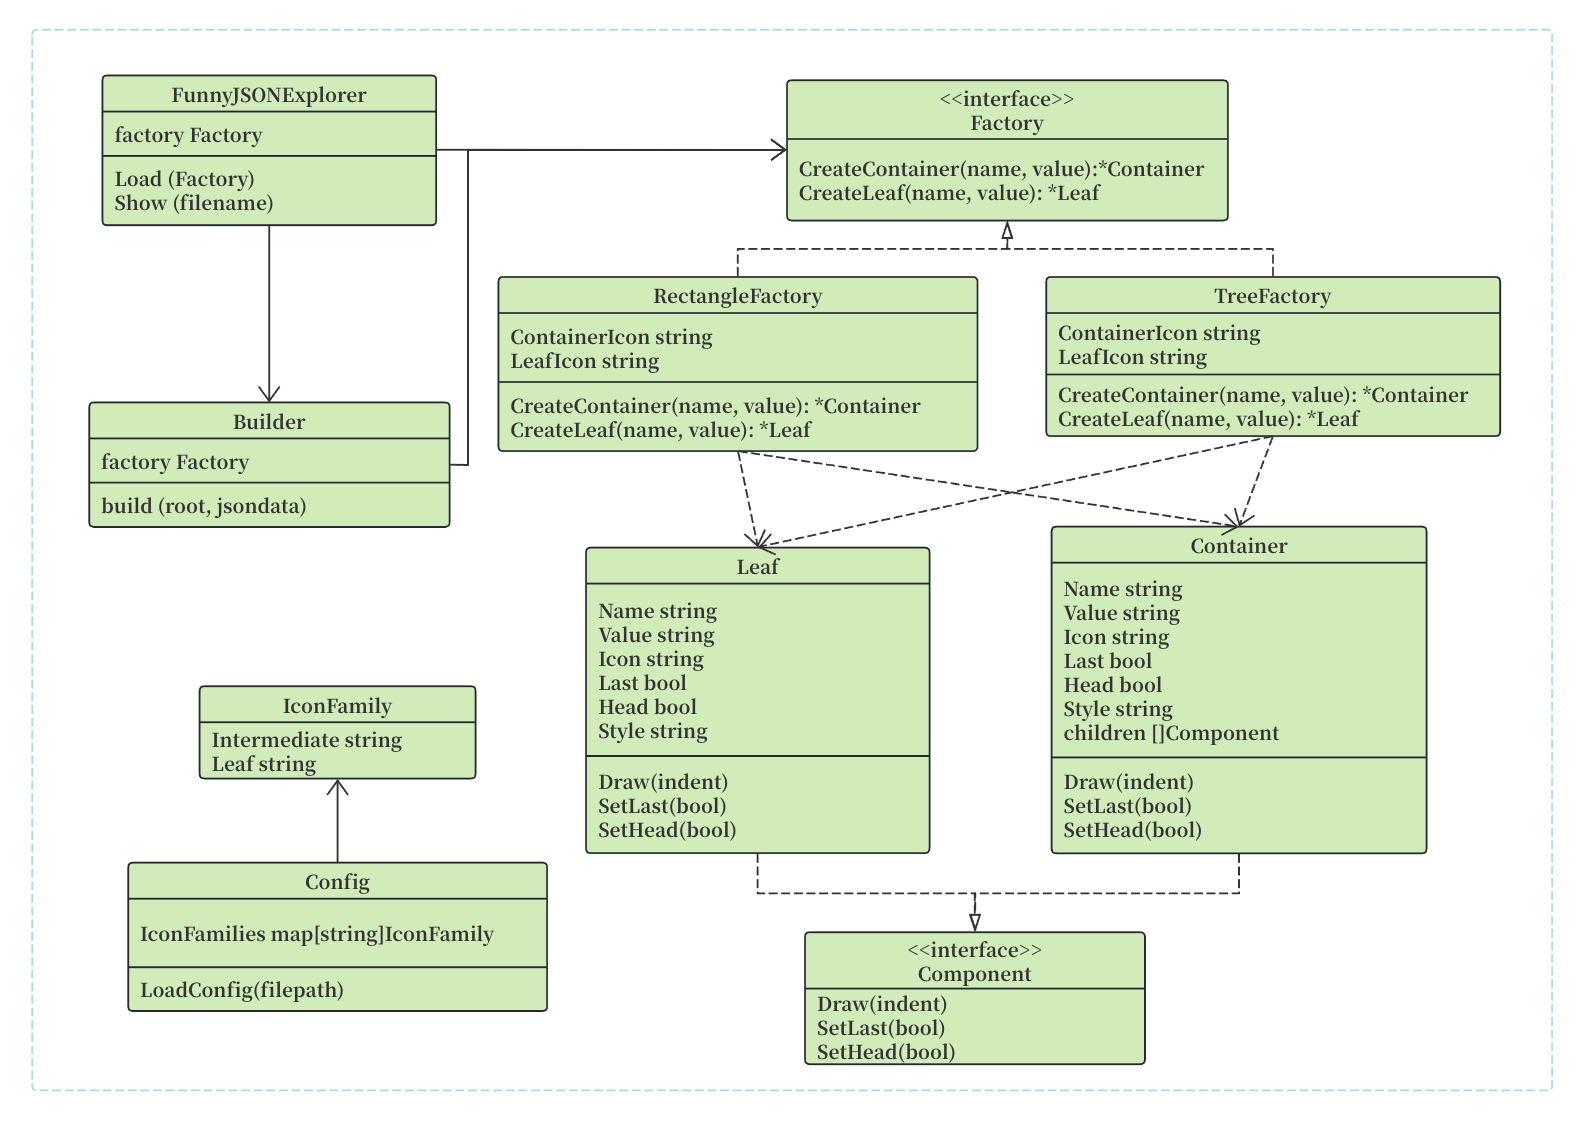
\includegraphics[width=1.1\textwidth]{figures/uml-class.png}
    \caption{FJE-GO项目的UML类图}
    \label{fig:uml}
\end{figure}

FJE-GO项目的UML类图如上图 \ref{fig:uml} 所示,其中类的命名参考了实验要求中的领域模型,下面对其进行具体说明。



\subsubsection{Funny JSON Explorer}
\begin{itemize}
    \item \textbf{描述:}
    \begin{itemize}
        \item 这是程序的主类,主要实现读取 JSON 文件并对其进行可视化的主过程。
        \item 其定义了一个factor的抽象工厂对象,主要目的是通过抽象工厂接口来接受main函数中根据具体风格指定的具体工厂对象(例如TreeFactory以及RectangleFactory)。
        \item 在对JSON文件的读取和创建过程中,为了将复杂的自定义Component结构的创建解耦,根据建造者设计模式可以创建一个Builder类,在builder类中会根据不同的工厂类型创建不同风格的树结构,从而将创建过程分离出去。
    \end{itemize}
    \item \textbf{主要方法:}
    \begin{itemize}
        \item \textbf{Load(factory Factory)}: 用来设置使用的抽象工厂对象。
        \item \textbf{Show(filename string)}: 读取JSON文件并进行可视化。具体来说,实现对指定路径下的JSON文件进行读取并调用Builder的build方法将JSON结构转换为自定义的Component结构,最后调用root节点的Draw方法进行可视化。
    \end{itemize}
\end{itemize}

\subsubsection{Builder}
\begin{itemize}
    \item \textbf{描述:}
    \begin{itemize}
        \item 主要实现根据 JSON 数据构建树结构,并返回创建的根节点,从而实现创建过程在主过程中的解耦。
    \end{itemize}
    \item \textbf{属性:}
    \begin{itemize}
        \item factory: 创建节点所使用的工厂,可以根据具体工厂类型进行创建。
    \end{itemize}
    \item \textbf{方法:}
    \begin{itemize}
        \item \textbf{Build(root Component, data map[string]interface{})}: 基于JSONdata以及传入的引用根节点进行树结构的创建。采用的方法是DFS思想,通过深度优先遍历整个JSON结构创建所有中间节点Container以及叶节点Leaf,最后返回根节点。
    \end{itemize}
\end{itemize}

\subsubsection{Factory}
\begin{itemize}
    \item \textbf{描述:}
    \begin{itemize}
        \item 这是抽象工厂接口,用于创建中间节点Container和叶子节点Leaf。这是一种抽象工厂设计模式的思想,可以通过抽象接口来支持新的Style以及新的具体工厂类型,实现良好的可扩展性。
    \end{itemize}
    \item \textbf{方法:}
    \begin{itemize}
        \item \textbf{CreateContainer(name string, value string) *Container}: 通过节点键值创建一个中间节点。
        \item \textbf{CreateLeaf(name string, value string) *Leaf}: 通过节点键值对创建一个叶子节点。
    \end{itemize}
\end{itemize}

\subsubsection{TreeFactory 和 RectangleFactory}
\begin{itemize}
    \item \textbf{描述:}
    \begin{itemize}
        \item Factory 接口的具体实现,用于创建特定Style的节点。
    \end{itemize}
    \item \textbf{属性:}
    \begin{itemize}
        \item ContainerIcon: 中间节点图标,用于在可视化指定具体的中间节点使用的图标。
        \item LeafIcon: 叶子节点图标,用于在可视化指定具体的叶子节点使用的图标。
    \end{itemize}
    \item \textbf{方法:}
    \begin{itemize}
        \item \textbf{CreateContainer(name string, value string) *Container}: 通过节点键值创建一个具体Style的中间节点。
        \item \textbf{CreateLeaf(name string, value string) *Leaf}: 通过节点键值创建一个具体Style的叶子节点。
    \end{itemize}
\end{itemize}

\subsubsection{Component}
\begin{itemize}
    \item \textbf{描述:}
    \begin{itemize}
        \item 抽象节点接口类型,用于确保节点的继承可以实现Draw方法。
    \end{itemize}
    \item \textbf{方法:}
    \begin{itemize}
        \item \textbf{Draw(indent string)}: 递归实现节点可视化,其中indent为递归传递的可视化前缀。
        \item \textbf{SetLast(b bool)}: 设置是否为最后一个子节点。
        \item \textbf{SetHead(b bool)}: 设置是否为头节点。
    \end{itemize}
\end{itemize}

\subsubsection{Leaf}
\begin{itemize}
    \item \textbf{职责:}
    \begin{itemize}
        \item 是对抽象节点类型的具体实现,表示一个树结构中的叶子节点。
    \end{itemize}
    \item \textbf{属性:}
    \begin{itemize}
        \item icon: 叶子节点使用的图标类型。
        \item name: 叶子节点的名称。
        \item Head: 是否为头节点,用于可视化判断。
        \item Last: 是否为尾节点,用于可视化判断。
    \end{itemize}
    \item \textbf{方法:}
    \begin{itemize}
        \item \textbf{Draw(indent string)}: 根据前缀indent可视化叶子节点。
        \item \textbf{SetHead(b bool)}: 设置是否为头节点。
        \item \textbf{SetLast(b bool)}: 设置是否为尾节点。
    \end{itemize}
\end{itemize}

\subsubsection{Container}
\begin{itemize}
    \item \textbf{职责:}
    \begin{itemize}
        \item 是对抽象节点类型的具体实现,表示一个树结构中的中间节点,其拥有子节点列表。
    \end{itemize}
    \item \textbf{属性:}
    \begin{itemize}
        \item icon: 中间节点使用的图标类型。
        \item name: 中间节点的名称。
        \item Head: 是否为头节点,用于可视化判断。
        \item Last: 是否为尾节点,用于可视化判断。
        \item children: 中间节点的维护子节点列表。
    \end{itemize}
    \item \textbf{方法:}
    \begin{itemize}
        \item \textbf{Draw(indent string)}: 根据前缀indent可视化中间节点。
        \item \textbf{AddChild(child Component)}: 为中间节点添加子节点。
        \item \textbf{SetHead(b bool)}: 设置是否为头节点。
        \item \textbf{SetLast(b bool)}: 设置是否为最后一个子节点。
    \end{itemize}
\end{itemize}

\subsubsection{IconFamily}
\begin{itemize}
    \item \textbf{描述:}
    \begin{itemize}
        \item 用于表示所使用的图表族,主要包括对中间节点或者叶子节点两种不同的Icon。
    \end{itemize}
    \item \textbf{属性:}
    \begin{itemize}
        \item Intermediate: 中间节点图标。
        \item Leaf: 叶节点图标。
    \end{itemize}
\end{itemize}

\subsubsection{Config}
\begin{itemize}
    \item \textbf{描述:}
    \begin{itemize}
        \item 主要用于存储在config.json文件中所指定的所有图标族,导入给main函数用于用户选取。
    \end{itemize}
    \item \textbf{属性:}
    \begin{itemize}
        \item IconFamilies: 所有配置图表族组,用map[string]IconFamily存储。
    \end{itemize}
    \item \textbf{方法:}
    \begin{itemize}
        \item \textbf{LoadConfig(filePath string) (*Config, error)}: 从config.json文件导入所有的图标族,加载至本地的IconFamilies中。
    \end{itemize}
\end{itemize}















\subsection{设计模式}
\subsubsection{工厂方法模式}
工厂方法模式(Factory Method Pattern)是一种创建型设计模式,提供了一种创建对象的接口,但由子类决定要实例化的类是哪一个。以此试图将对象的实例化推迟到子类。它主要用于解决对象创建的问题,通过将对象创建的细节封装起来,使得客户端代码无需知道具体的创建过程。

在本FJE-GO项目中,工厂方法模式用于创建不同风格的节点对象,包括中间节点(Container)和叶子节点(Leaf)。
具体来说,定义了一个抽象工厂接口 Factory,如下:
\begin{lstlisting}
type Factory interface {
    CreateContainer(name, value string) *Container
    CreateLeaf(name, value string) *Leaf
}
\end{lstlisting}

并提供了两个具体的实现 TreeFactory和RectangleFactory,分别用于创建树形风格和矩形风格的节点。下面给出了TreeFactory的具体代码实现:

\begin{lstlisting}
type TreeFactory struct {
	ContainerIcon string
	LeafIcon      string
}

func (f *TreeFactory) CreateContainer(name string, value string) *Container {
	return &Container{Name: name, Value: value, Icon: f.ContainerIcon, Style: "tree", Last: false}
}

func (f *TreeFactory) CreateLeaf(name string, value string) *Leaf {
	return &Leaf{Name: name, Value: value, Icon: f.LeafIcon, Style: "tree", Last: false}
}
\end{lstlisting}

在客户端可以通过不同的风格类型创建不同的工厂来实现可拓展性,符合开闭原则。
\begin{lstlisting}
// style-dealing
var factory Factory
switch *style {
case "tree":
    factory = &TreeFactory{icon.Intermediate, icon.Leaf}
case "rectangle":
    factory = &RectangleFactory{icon.Intermediate, icon.Leaf}
//TODO: 在这里可以添加新的样式的抽象工厂
default:
    fmt.Println("Unknown style")
    return
}
\end{lstlisting}

\subsubsection{建造者模式}

建造者模式(Builder Pattern)主要用于将一个复杂对象的构建与表示分离,使得同样的构建过程可以创建不同的表示。

在本FJE-GO项目中使用了建造者设计模式的思想,通过Builder 类来负责根据 JSON 数据构建树结构,并返回根节点,从而实现在JSE主过程中将构建过程解耦。

\begin{lstlisting}
type Builder struct {
	factory Factory
}

// Build方法 根据 JSON 数据构建树结构,返回根节点
func (b *Builder) Build(root Component, data map[string]interface{}) {
	for key, value := range data {
		var child Component
		if _, ok := value.(map[string]interface{}); ok {
			child = b.factory.CreateContainer(key, val)
			root.(*Container).AddChild(child)
		} else {
			// Leaf and NoneTy
			child := b.factory.CreateLeaf(key, val)
			root.(*Container).AddChild(child)
		}

		if v, ok := value.(map[string]interface{}); ok {
			b.Build(child, v)
		}
	}
}
\end{lstlisting}

优势在于通过建造者模式可以将构建过程解耦分离并封装,从而可以根据不同的 JSON 数据构建不同的树结构,而不需要修改构建过程的代码;另外,它提供了更加良好的扩展性,由于建造者模式将构建过程进行了封装,可以更容易地扩展构建过程。


\subsubsection{组合模式}
组合模式(Composite Pattern)是一种结构型设计模式,它允许将对象组合成树形结构以表示“部分-整体”的层次结构。使用组合模式可以很好地利用递归和多态的机制来使用树形结构。在本FJE-GO项目中,Container 类表示树形结构中的中间节点,Leaf类表示叶子节点,它们共同实现了 Component 接口。其中,Container作为中间节点拥有children数据结构,其有Component组合而成。代码如下:

\begin{lstlisting}
type Component interface {
	Draw(string)
	SetLast(bool) /
	SetHead(bool)
}

type Container struct {
	Name     string
	Value    string
	Icon     string
	Last     bool 
	Head     bool
	Style    string
	Children []Component
}
\end{lstlisting}

对于JSON结构(树形结构),使用组合模式允许在节点中包含其他节点,从而可以递归地构建复杂的树形结构。通过将 Container类中的 Children属性设置为 Component 接口的实现类,实现了树形结构的递归组合,从而用简单的节点类型实现负责树形整体。































\section{效果截图}

使用如下简单的JSON代码可以进行测试:

\begin{lstlisting}
{
  "oranges": {
    "mandarin": {
      "clementine": null,
      "tangerine": "cheap & juicy!"
    }
  },
  "apples": {
    "gala": null,
    "pink lady": null
  }
}
\end{lstlisting}

使用两种图标族(weather以及poker)以及两种风格(tree以及rectangle)效果如下:


\begin{figure}[htbp]
\centering
\begin{minipage}[t]{0.48\textwidth}
    \centering
    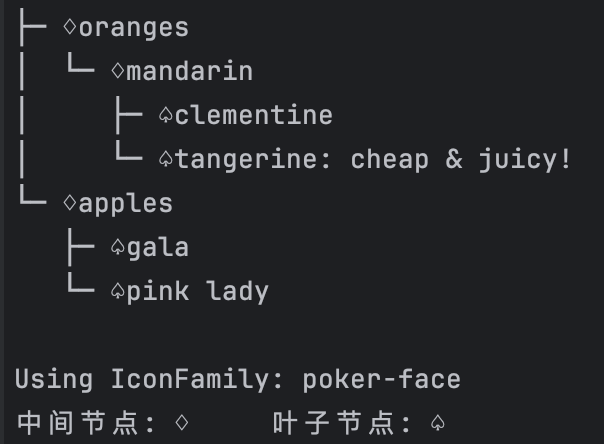
\includegraphics[width=\textwidth]{figures/tre-pok.png}
    \caption{Tree-Style Poker-Icon JSON可视化}
    \label{fig:tre-pok}
\end{minipage}
\hfill
\begin{minipage}[t]{0.48\textwidth}
    \centering
    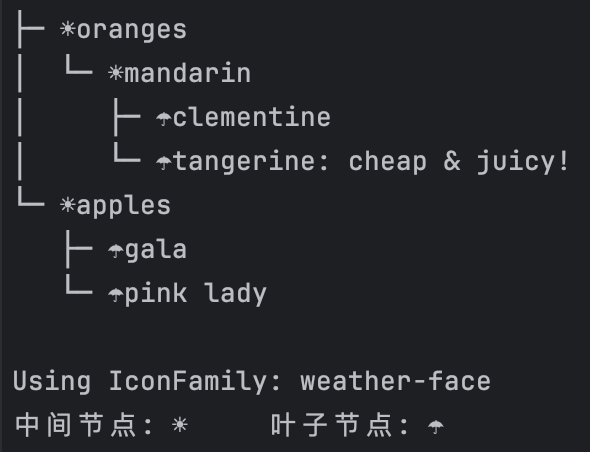
\includegraphics[width=\textwidth]{figures/tre-wea.png}
    \caption{Tree-Style Weather-Icon JSON可视化}
    \label{fig:tre-wea}
\end{minipage}
\end{figure}


\begin{figure}[htbp]
\centering
\begin{minipage}[t]{0.48\textwidth}
    \centering
    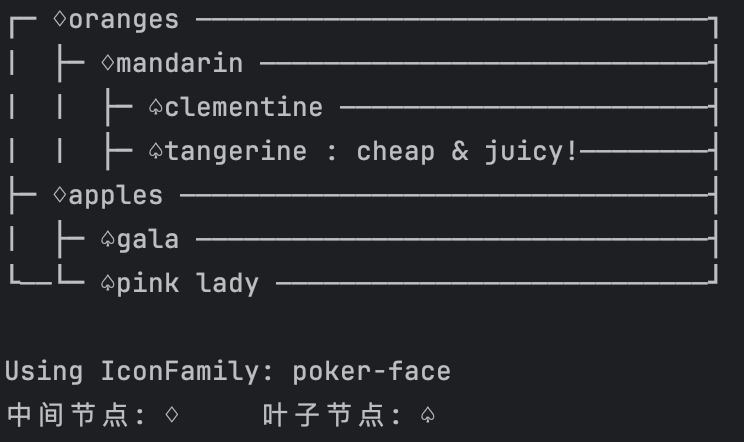
\includegraphics[width=\textwidth]{figures/rec-pok.png}
    \caption{Rectangle-Style Poker-Icon JSON可视化}
    \label{fig:rec-pok}
\end{minipage}
\hfill
\begin{minipage}[t]{0.48\textwidth}
    \centering
    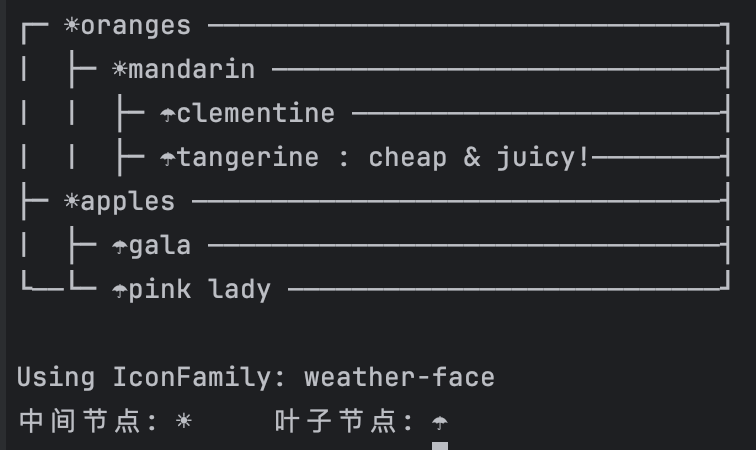
\includegraphics[width=\textwidth]{figures/rec-wea.png}
    \caption{Rectangle-Style Weather-Icon JSON可视化}
    \label{fig:rec-wea}
\end{minipage}
\end{figure}


为了验证可视化效果的正确性,可以使用层数更加深的文件进行可视化,如图 \ref{fig:deep-tre} 以及图 \ref{fig:deep-rec} 所示,可以看出效果是符合预期的。


\begin{figure}[htbp]
\centering
\begin{minipage}[t]{0.42\textwidth}
    \centering
    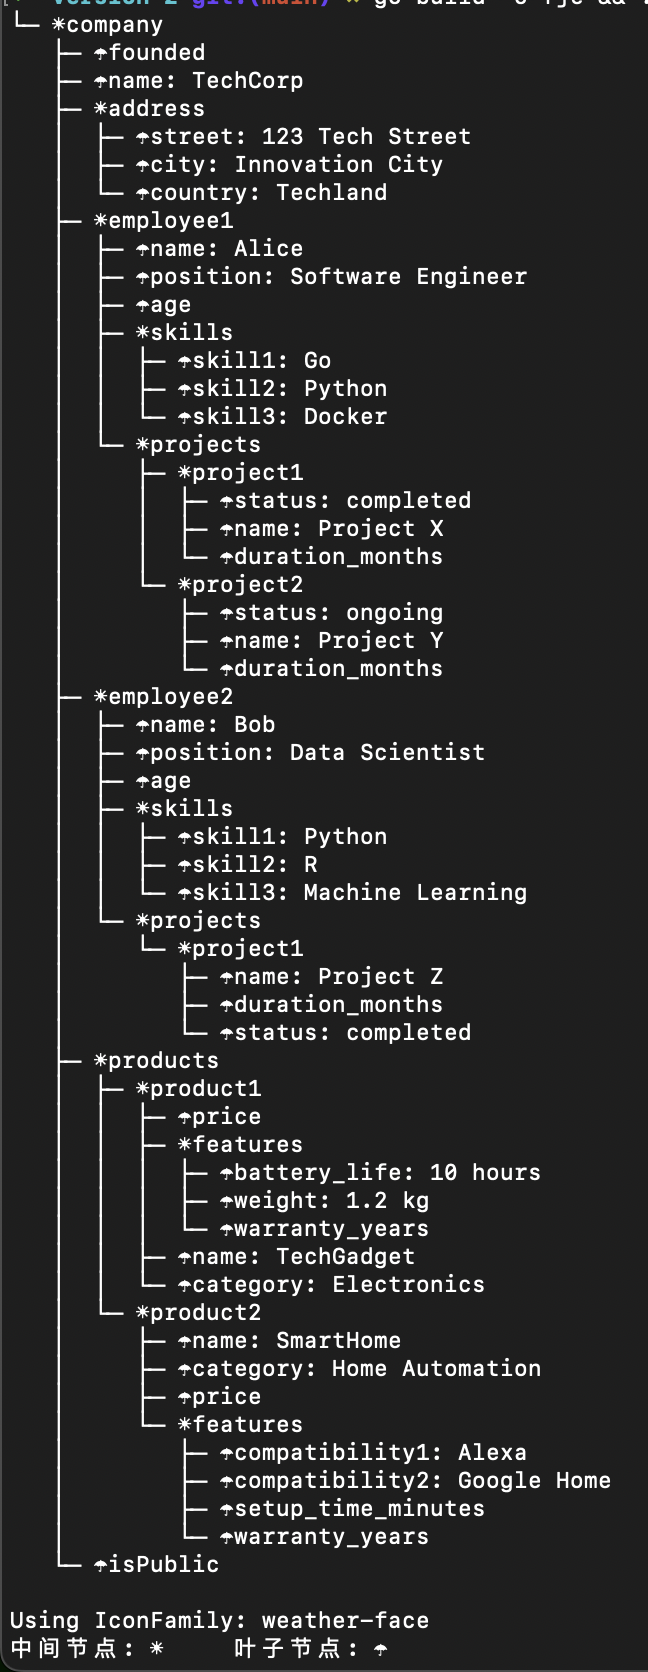
\includegraphics[width=\textwidth]{figures/deep-tre.png}
    \caption{加深的Tree-Style Weather-Icon JSON可视化效果}
    \label{fig:deep-tre}
\end{minipage}
\hfill
\begin{minipage}[t]{0.48\textwidth}
    \centering
    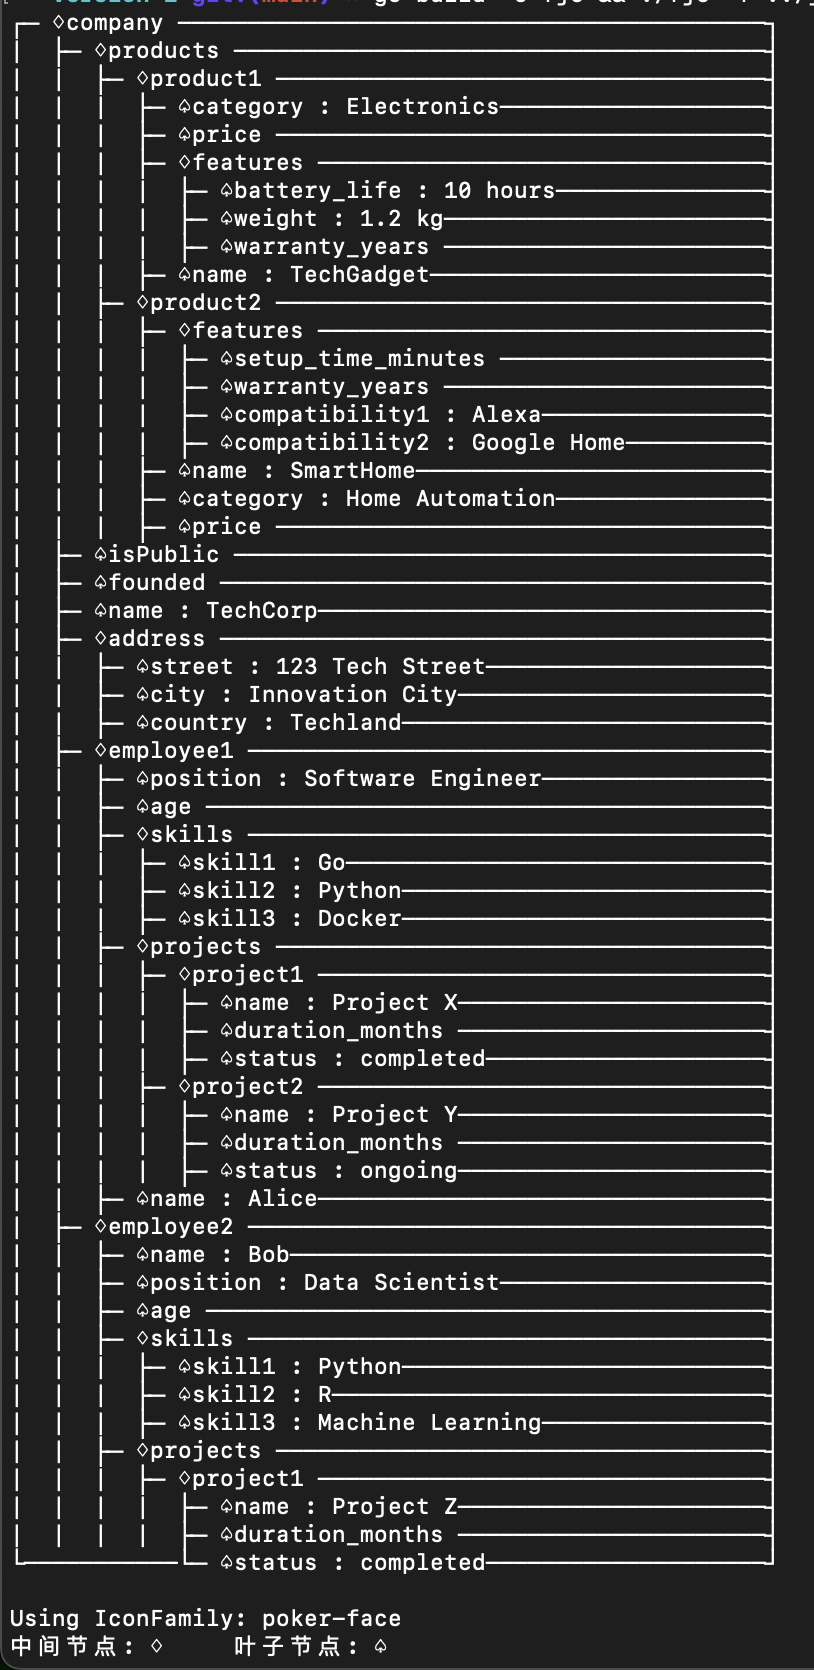
\includegraphics[width=\textwidth]{figures/deep-rec.png}
    \caption{加深的Rectangle-Style Pocker-Icon JSON可视化效果}
    \label{fig:deep-rec}
\end{minipage}
\end{figure}





%结束本文
\end{document}